\chapter{जंतु कहाँ रहते हैं}\label{ch:g2:where-animals-live}

स्कूल के अहाते में तुम्हें ट्राउट नहीं मिलेगी, और न ही तालाब की तह में
कोई गिलहरी। हर \omterm{def:g1:animals-around-us:animal}{जंतु} उसी तरह की जगह पर रहता है जो उसके लिए ठीक बैठती है
--- जहाँ उसे अपना भोजन, अपनी ओट और अपने पड़ोसी मिलते हैं।
जीवविज्ञानियों के पास \omterm{def:g1:animals-around-us:animal}{जंतु} की इस अपनी ज़मीन के लिए एक नाम है।

\section{आवास}

\begin{definition}[आवास]\label{def:g2:where-animals-live:habitat}
किसी \omterm{def:g1:animals-around-us:animal}{जंतु} का \emph{आवास}\index{आवास} वह तरह की जगह है जहाँ वह
स्वाभाविक रूप से रहता है और उसे हर ज़रूरी चीज़ मिलती है: भोजन, पानी,
ओट, और अपने बच्चों के लिए एक सुरक्षित कोना। तालाब, जंगल, मैदान, बाड़
और समुद्र-तट, सब आवास हैं।
\end{definition}

\begin{example}[चार आवास, चार मोहल्ले]\label{ex:g2:where-animals-live:four}
\emph{तालाब} में: मेंढक, व्याध-पतंगे, काँटा-मछलियाँ, तालाब के घोंघे।
\emph{जंगल} में: गिलहरियाँ, हिरन, कठफोड़वे, जंगली चींटियाँ।
\emph{मैदान} में: ख़रगोश, टिड्डे, तितलियाँ, खेत के चूहे। पुरानी
\emph{दीवार} के पत्थरों के नीचे: कठ-जूएँ, मकड़ियाँ, और कभी-कभी ऊपर धूप
सेंकती एक छिपकली।
\end{example}

\begin{omfigure}
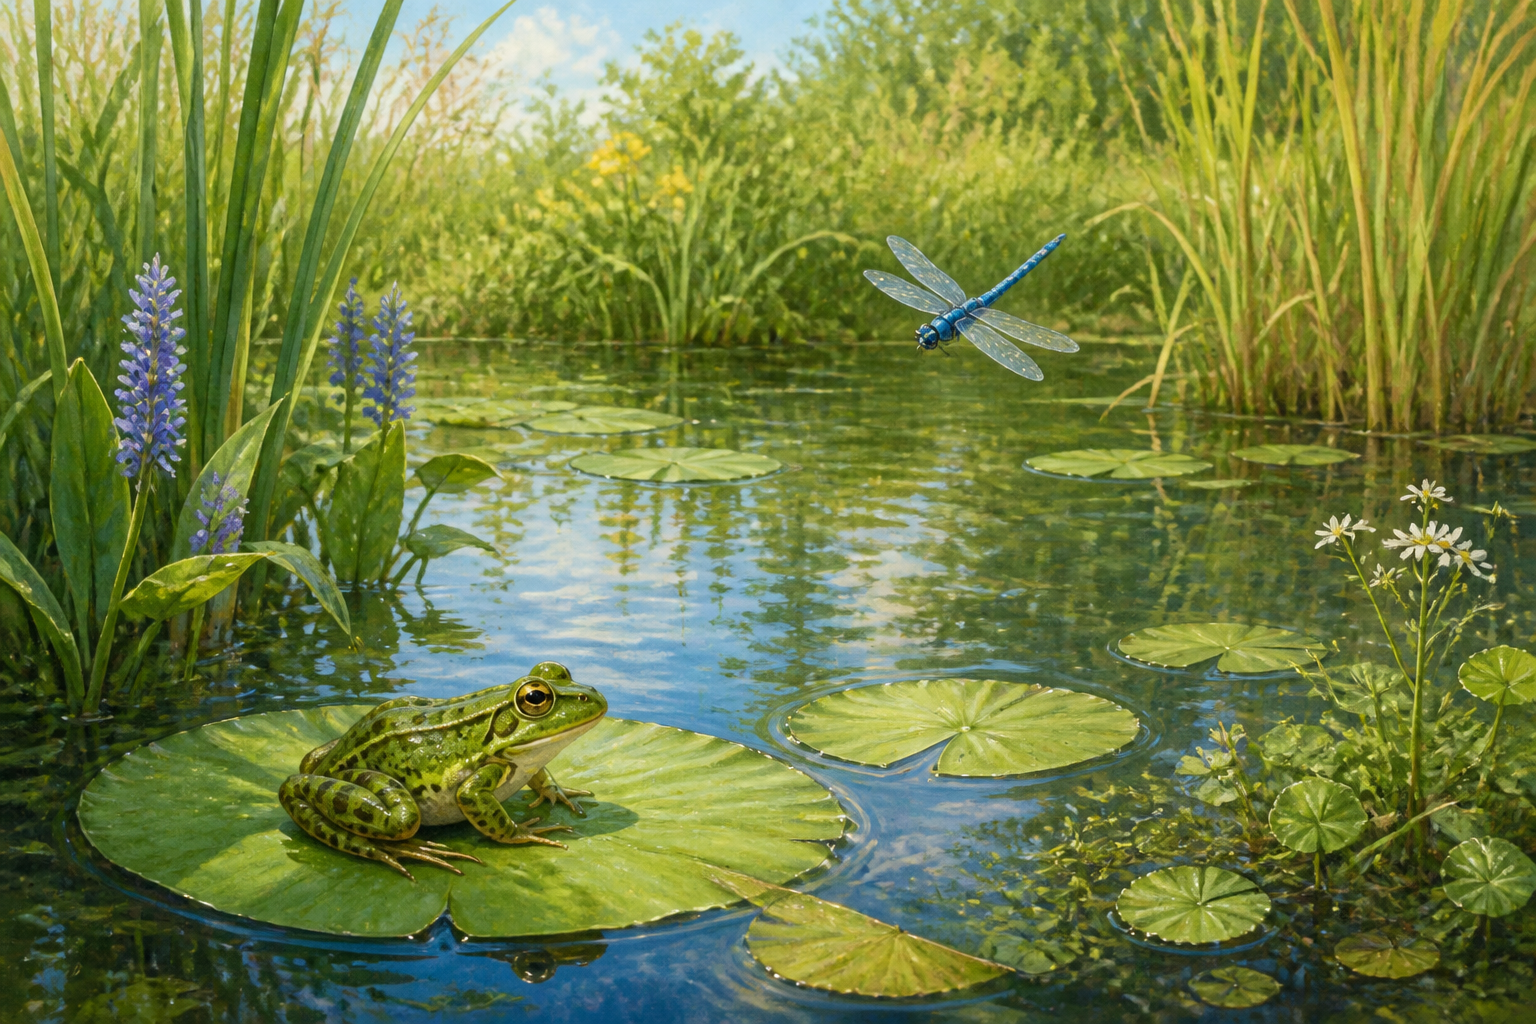
\includegraphics[width=0.62\linewidth]{images/book1/ai/g2-live-pond.png}

{\small तालाब का \omterm{def:g2:where-animals-live:habitat}{आवास} और उसके दो बाशिंदे अपने घर में: कुमुदिनी के पत्ते
पर एक मेंढक, और गश्त लगाता एक व्याध-पतंगा।}
\end{omfigure}

\begin{omfigure}
\begin{tikzpicture}[scale=0.88]
  \draw[thick, omDef, fill=omDef!7, rounded corners=6pt]
    (0,0) rectangle (3.4,2.6);
  \draw[thick, omMeth, fill=omMeth!7, rounded corners=6pt]
    (3.9,0) rectangle (7.3,2.6);
  \draw[thick, omProp, fill=omProp!7, rounded corners=6pt]
    (7.8,0) rectangle (11.2,2.6);
  \node[font=\small\bfseries, omDef] at (1.7,2.25) {तालाब};
  \node[font=\small\bfseries, omMeth] at (5.6,2.25) {जंगल};
  \node[font=\small\bfseries, omProp] at (9.5,2.25) {मैदान};
  \node[font=\small, align=center] at (1.7,1.05)
    {मेंढक\\ व्याध-पतंगा\\ काँटा-मछली};
  \node[font=\small, align=center] at (5.6,1.05)
    {गिलहरी\\ कठफोड़वा\\ हिरन};
  \node[font=\small, align=center] at (9.5,1.05)
    {ख़रगोश\\ टिड्डा\\ तितली};
\end{tikzpicture}

{\small तीन \omterm{def:g2:where-animals-live:habitat}{आवास} और उनके कुछ बाशिंदे। इन्हें आपस में बदलकर देखो ---
गिलहरी तालाब में ज़्यादा देर न टिकती।}
\end{omfigure}

\begin{remark}[एक आवास, कई घर]\label{rem:g2:where-animals-live:layers}
एक \omterm{def:g2:where-animals-live:habitat}{आवास} के कई कोने होते हैं। एक ही जंगल में कठफोड़वा तनों पर ऊँचाई पर
रहता है, गिलहरी शाखाओं में, हिरन झाड़ियों के बीच, और जंगली चींटियाँ
ज़मीन पर अपने ढेर जैसे घर में। वही जंगल, अलग-अलग मंज़िलें --- इसीलिए
बहुत-से \omterm{def:g1:animals-around-us:animal}{जंतु} बिना भीड़ किए एक ही \omterm{def:g2:where-animals-live:habitat}{आवास} बाँट सकते हैं।
\end{remark}

\section{आवास के अनुरूप ढला हुआ}

\begin{proposition}[जंतु अपने आवास से मेल खाते हैं]\label{prop:g2:where-animals-live:fit}
\omterm{def:g1:animals-around-us:animal}{जंतु} का शरीर और उसकी आदतें उसकी रहने की जगह से मेल खाती हैं:
\begin{itemize}
  \item मेंढक के झिल्लीदार पैर पानी को धकेलते हैं --- तालाब के लिए
        बने;
  \item गिलहरी के पकड़ने वाले पंजे और संतुलन बनाती बड़ी पूँछ \omterm{def:g1:plants-around-us:tree}{पेड़ों} के
        लिए बने हैं;
  \item ख़रगोश के खोदने वाले पंजे और चेतावनी सुनते लंबे \omterm{def:g1:the-five-senses:sense}{कान} खुले मैदान
        और नीचे बनी बिलों के लिए बने हैं;
  \item बत्तख़ के \omterm{def:g1:animals-around-us:covering}{पंख} पानी बहा देते हैं, और उसके झिल्लीदार पैर खेते
        हैं।
\end{itemize}
ग़लत \omterm{def:g2:where-animals-live:habitat}{आवास} में पहुँचते ही \omterm{def:g1:animals-around-us:animal}{जंतु} ये सारे फ़ायदे खो देता है।
\end{proposition}
\admitted

\begin{example}[छछूँदर का साज़-सामान]\label{ex:g2:where-animals-live:mole}
छछूँदर ज़मीन के नीचे रहता है, मैदान के नीचे ख़ुद खोदी सुरंगों में।
उसके हाथ चौड़े खोदने वाले फावड़े हैं, उसके \omterm{def:g1:animals-around-us:covering}{रोम} दोनों दिशाओं में चपटे
लेटते हैं ताकि मिट्टी उन्हें कभी उलझा न सके, और अँधेरे में उसकी कमज़ोर
\omterm{def:g1:the-five-senses:sense}{आँखों} से कोई ख़ास फ़र्क़ नहीं पड़ता। ज़मीन के ऊपर वह भद्दा है; अपने
\omterm{def:g2:where-animals-live:habitat}{आवास} में वह उस्ताद है।
\end{example}

\begin{method}[जंतु को उसके आवास से मिलाना]\label{met:g2:where-animals-live:matching}
कोई अनजान \omterm{def:g1:animals-around-us:animal}{जंतु} मिले, तो:
\begin{enumerate}
  \item उसका साज़-सामान देखो: झिल्लीदार पैर? पंजे? डैने? खोदने वाले
        पंजे?
  \item पूछो कि वह क्या खाता है, और वह भोजन कहाँ मिलता है;
  \item पूछो कि वह कहाँ ओट ले सकता है और बच्चे पाल सकता है;
  \item जो \omterm{def:g2:where-animals-live:habitat}{आवास} तीनों का उत्तर देता है, वही उसका संभावित घर है।
\end{enumerate}
\end{method}

\section{आवास खो भी सकते हैं}

\begin{proposition}[आवास नहीं, तो बाशिंदे नहीं]\label{prop:g2:where-animals-live:loss}
\omterm{def:g1:animals-around-us:animal}{जंतु} अपने \omterm{def:g2:where-animals-live:habitat}{आवास} के बिना नहीं जी सकता। कोई तालाब पाट दिया जाए तो उसके
मेंढक और व्याध-पतंगे उसी के साथ ग़ायब हो जाते हैं; कोई बाड़ उखाड़ दी
जाए तो वहाँ घोंसला बनाने वाले पक्षी अपनी ओट खो देते हैं। \omterm{def:g1:animals-around-us:animal}{जंतुओं} की
रक्षा उनकी रहने की जगहों की रक्षा से शुरू होती है।
\end{proposition}
\admitted

\begin{example}[स्कूल का तालाब]\label{ex:g2:where-animals-live:schoolpond}
एक स्कूल अपने अहाते के कोने में छोटा-सा तालाब खोदता है। दो साल के
भीतर उस पर व्याध-पतंगे गश्त लगाते हैं, पानी पर जल-चींटे चलते हैं, और
मेंढक आकर बस जाते हैं --- उन्हें कोई लाया नहीं। \omterm{def:g2:where-animals-live:habitat}{आवास} बना दो, और
बाशिंदे ख़ुद उसे ढूँढ़ लेते हैं।
\end{example}

\begin{remark}[बिना खलल डाले देखना]\label{rem:g2:where-animals-live:respect}
किसी \omterm{def:g2:where-animals-live:habitat}{आवास} में जाकर हम मेहमान होते हैं। चुपचाप देखो, उलटे हुए पत्थर
वैसे ही वापस रखो जैसे मिले थे, \omterm{def:g2:animals-grow-up:born}{अंडों} और घोंसलों को हाथ मत लगाओ, और
अपना कूड़ा घर ले जाओ --- \omterm{def:g2:where-animals-live:habitat}{आवास} को यह भूल ही जाना चाहिए कि तुम वहाँ थे।
अगले अध्याय प्रकृति की देखभाल के और तरीक़े बताते हैं।
\end{remark}

\section{अभ्यास}

\begin{exercise}[$\star$]\label{exo:g2:where-animals-live:1}
\omterm{def:g2:where-animals-live:habitat}{आवास} क्या है? \omterm{def:g1:animals-around-us:animal}{जंतु} को उसमें मिलने वाली चार चीज़ों के नाम बताओ।
\end{exercise}

\begin{exercise}[$\star$]\label{exo:g2:where-animals-live:2}
तालाब के दो \omterm{def:g1:animals-around-us:animal}{जंतु} बताओ, जंगल के दो, और मैदान के दो।
\end{exercise}

\begin{exercise}[$\star$]\label{exo:g2:where-animals-live:3}
हर \omterm{def:g1:animals-around-us:animal}{जंतु} के लिए कौन-सा \omterm{def:g2:where-animals-live:habitat}{आवास} ठीक बैठता है: काँटा-मछली, कठफोड़वा, टिड्डा,
कठ-जूँ?
\end{exercise}

\begin{exercise}[$\star$]\label{exo:g2:where-animals-live:4}
मेंढक का तैरने वाला साज़-सामान क्या है? और गिलहरी का \omterm{def:g1:plants-around-us:tree}{पेड़} चढ़ने वाला?
\end{exercise}

\begin{exercise}[$\star$]\label{exo:g2:where-animals-live:5}
\cref{ex:g2:where-animals-live:mole} से छछूँदर के भूमिगत साज़-सामान की
तीन चीज़ें गिनाओ।
\end{exercise}

\begin{exercise}[$\star$]\label{exo:g2:where-animals-live:6}
\cref{rem:g2:where-animals-live:layers} में हर \omterm{def:g1:animals-around-us:animal}{जंतु} जंगल की कौन-सी
``मंज़िल'' इस्तेमाल करता है: कठफोड़वा, गिलहरी, हिरन, जंगली चींटी?
\end{exercise}

\begin{exercise}[$\star$]\label{exo:g2:where-animals-live:7}
तालाब पाट दिए जाने पर मेंढकों और व्याध-पतंगों का क्या होता है? इससे
\omterm{def:g1:animals-around-us:animal}{जंतुओं} की रक्षा के बारे में क्या सीख मिलती है?
\end{exercise}

\begin{exercise}[$\star$]\label{exo:g2:where-animals-live:8}
करके देखो: अपने आस-पास कोई एक छोटा \omterm{def:g2:where-animals-live:habitat}{आवास} चुनो --- किसी पत्थर के नीचे,
कोई झाड़ी, कोई क्यारी। चुपचाप देखो और तय समय में दिखने वाले हर \omterm{def:g1:animals-around-us:animal}{जंतु} की
सूची बनाओ। हर पत्थर वापस रख दो। तुम्हारे नन्हे \omterm{def:g2:where-animals-live:habitat}{आवास} में कितने बाशिंदे
थे?
\end{exercise}

\begin{exercise}[$\star\star$]\label{exo:g2:where-animals-live:9}
पहेली वाले एक \omterm{def:g1:animals-around-us:animal}{जंतु} के झिल्लीदार पैर हैं, पानी बहा देने वाले घने \omterm{def:g1:animals-around-us:covering}{पंख}
हैं, और छानने वाली चपटी चोंच है।
\cref{met:g2:where-animals-live:matching} से उसका \omterm{def:g2:where-animals-live:habitat}{आवास} बताओ --- और
शायद \omterm{def:g1:animals-around-us:animal}{जंतु} भी।
\end{exercise}

\begin{exercise}[$\star\star$]\label{exo:g2:where-animals-live:10}
टॉम एक मेंढक की ``मदद'' करना चाहता है और उसे घर ले जाकर भरपूर भोजन
वाले सूखे काँच-घर में रखना चाहता है।
\cref{prop:g2:where-animals-live:fit} और
\cref{prop:g2:where-animals-live:loss} से समझाओ कि इससे मेंढक का
ज़रा भी भला नहीं होगा।
\end{exercise}
